
For scalar regression problems, one solution to specifying validity of CFs is to set a threshold $\varepsilon$, so that the $\mathrm{CF}$ set is $\mathcal{S} \doteq$ $\{x \in \mathcal{X}:|f(x)-f(q)| \geq \varepsilon\}$. This construction yields an equivalency between instances of CFX-EXISTENCE for (binary) classifiers and regressors. They are also tractable, since the targets are defined using preorders, which admit trivial verification circuits. However, thresholding does not distinguish between $\mathrm{CFs}$ in $\mathcal{S}$, which is a problem when the distance in $x$ far exceeds $\varepsilon$, leading to unrealistic CFs that are far from the query point.

\begin{figure}[h]
    \centering
    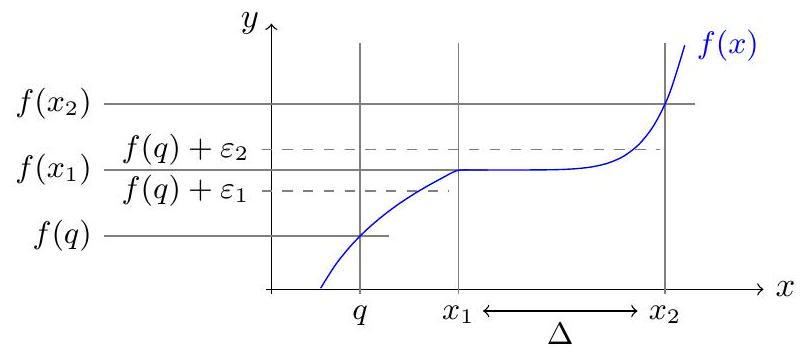
\includegraphics[width=0.4\textwidth]{images/potential.jpg}
    \caption{Threshold robustness issue with CFEs: choosing $\varepsilon_{2}$ over $\varepsilon_{1}$ yields $x_{2}$ rather than $x_{1}$ as the counterfactual.}
\end{figure}

 Furthermore, CFs defined via thresholding can be very sensitive to $\varepsilon$. Figure 1 shows an example where the query instance $q \in \mathcal{X}$ is bounded above by $q<x_{1}<x_{2}$, and $f$ is monotone increasing such that $f(q)<f(q)+\varepsilon_{1}<f\left(x_{1}\right)<f(q)+\varepsilon_{2}<f\left(x_{2}\right)$ for $0<\varepsilon_{1}<\varepsilon_{2}$. Define $\Delta \doteq x_{2}-x_{1}$. Setting $\varepsilon_{1}$ as the threshold yields the CF $x_{1}$, whereas choosing $\varepsilon_{2}$ yields $x_{2}$ instead. Considering the distance When $\Delta$ is large, $x_{2}$ is further from $q$ than $x_{1}$ is, and thus $\varepsilon_{2}$ is arguably a worse threshold than $\varepsilon_{1}$. as it yields CFs far from the query point. However, there is no ex ante way to choose between $\varepsilon_{1}$ and $\varepsilon_{2}$, which causes this threshold robustness issue. A key contribution our work is to formalise the notion of regression counterfactuals in terms of potentials instead of the direct instantiation of the primal-dual spaces via thresholds, which we will now describe.

\subsection*{Potential-Based Search}
In this work, we focus on a subset of $\mathbb{T}_{q}^{f}$ where, for a given query $q \in \mathcal{X}$, we ascribe to each output $y \in \mathcal{Y}$ a scalar potential which quantifies the value associated with candidate counterfactual points. This concept is closely related to the construction used in potential games [37] to analyse equilibria when agents' incentives are dictated by a single global function. Definition 2.3 below formalises this.
\begin{definition}
(Potential). A counterfactual potential function is an element $\rho$ of the set

$$
\mathcal{R}_{q}^{f} \doteq\left\{\rho \in C_{L}^{1}(\mathcal{Y}, \mathbb{R}): \max _{x \in \mathcal{X}} \rho(f(x))-\rho(f(q))>0\right\}
$$

of all continuously differentiable maps between model outputs and the real line, where $(f, q)$ is a model-query pair, $\rho$ and $\nabla \rho$ are $L$-Lipschitz, and the value of $\rho$ is not maximized at $q$.
\end{definition}